\documentclass[12pt, letterpaper]{article}
\usepackage[utf8]{inputenc}
\usepackage{graphicx}
\usepackage{hyperref}

\graphicspath{ {./images/} }

\title{My Math Notes}
\author{John Lockwood \thanks{Special thanks to my lovely wife}}
\date{June 2022}

\newcommand\T{\rule{0pt}{8mm}}       % Top strut

\begin{document}

\maketitle

\section{Introduction}

What I want to be able to do is to keep important math notes handy.
The goal of all this is to take the \href{https://clep.collegeboard.org/clep-exams/calculus}{Calculus CLEP Exam}.  
One approach to this is the \href{https://courses.modernstates.org/courses/course-v1:ModernStatesX+Calculus+2017/course/}{Modern States Course}
\section{Modern States Notes}
\subsection{Module 1, Limits}

Continuity is essential to calculus

Epsilon/delta formal def of Limits

Limits are central to def of both derivative and integrals.

Limits happen at a certain point, not for whole function.

Technical (epsilon/delta) definition of limits given \href{https://courses.modernstates.org/courses/course-v1:ModernStatesX+Calculus+2017/courseware/8f598eefb77a4cceb9d65d6ae993c417/4c2b909e818e421ba4a9e7aa31aba97f/?child=first}{here}

Limits might not exist

Function is continuous if f(x) exists \(\lim_{y \to x} f(x)\)  = f(x)

He's not going to do left and right limits.

To get limit, evaluating function only works for continuous functions.

Polynomials are continuous, rational functions are more tricky.  For example:

\[
    \lim_{x \to -1}\frac{x^2 + 2x + 1}{x + 1}
\]

limit by subst. is 0/0, which could be zero, one, infinity.  Indeterminate form.

Can do it by factoring out x+1, and cancel one out.

If get zero over zero, need to factor.

\vspace{5mm}

Another example: \(
    \lim_{x \to 0}\frac{1}{x}
\)

\vspace{5mm}
Limit does not exist!  DNE.

Watch out too for absolute value of x over x -- no limit, because diff for pos and neg values.

Note not all piecewise functions are discontinuous.

General rules for continuous functions:

Polynomials, exponential functions, and sin and cos are continuous.
Rational functions are continuous except at points where denominator is zero.
Logarithm is continuous, because domain is only (0,infinity)
Tangent function is discontinuous

\vspace{1cm}
Classic function that uses the squeeze theorem (memorize):
\(\lim{x \to 0}\frac{sin(x)}{x}\)
Answer ends up being one c.f. (Here's a \href{http://ime.math.arizona.edu/g-teams/Profiles/JS/Calc/SqueezeTheorem.pdf}{proof}.)

\subsection{Theory of the Derivative}
Derivative is scope of tangent line.
A tangent line intersects function at only one point.
Tangent lines -- are consructed of the limit of secant lines (a line that intersects at exactly two points)
\vspace{.5cm}

Definition of derivative:

\vspace{.5cm}

$f^\prime{(x)} = \lim_{h \to 0} \frac{f(x + h) - f(x)}{h}   $


So derivative is defined in terms of a limit.

As we shrink average rate of change to zero, we get derivative, which is instantaneous rate of change.

\section{Things to Research, Things To Memorize, Preliminaries}
\subsection{Things to Research}
\href{https://www.khanacademy.org/math/algebra/x2f8bb11595b61c86:functions/x2f8bb11595b61c86:inverse-functions-intro/v/introduction-to-function-inverses}{Inverse functions}

\subsection{Things To Memorize}
\subsection{Calculus Derivative Rules}
\subsubsection{Derivatives of log functions}
Derivative of Natural log of x:
\[\frac{d}{dx}[\ln x] = \frac{1}{x} \]
Derivative of log in another base is 
\[\frac{d}{dx}[\log_{a} x] = \frac{1}{(\ln a) x} \]
For example:
\[\frac{d}{dx}[\log_{10} x] = \frac{1}{(\ln 10) x} \]
For video showing this, see \href{https://www.khanacademy.org/math/in-in-grade-12-ncert/xd340c21e718214c5:continuity-differentiability/xd340c21e718214c5:logarithmic-functions-differentiation/v/logarithmic-functions-differentiation-intro}{Derivative of of log at any base of x}
\subsubsection{Derivatives of inverse functions:} 
(Notes on 
\href{https://www.khanacademy.org/math/differential-calculus/dc-chain/dc-inverse-func-diff/v/derivatives-of-inverse-functions-implicit?modal=1}{Kahn academy video}.)

Given: $f(x)$ and $g(x)$ are inverses, i.e. \[g(x) = f^-1(x)\]
then \textbf{the derivative of the inverse of $f(x)$ is given as follows}:
\[g'(x) = \frac{1}{f'(g(x))}\]
"This comes straight out of the chain rule."  Proof:
\[f(g(x)) = x\] 
(by inverse definition), therefore we can derviative of both sides:
\[ \frac{d}{dx} f(g(x)) = \frac{d}{dx} x\]
by Chain rule we get:
\[f'(g(x))*g'(x) = 1 \]
therefore, just divide both sides by $f'(x)$ to get
\[g'(x) = \frac{1}{f'(g(x))}\]
\subsubsection{Derviatives of basic trig functions}
\[\frac{d}{dx} sin(x) = cos(x)\]
\[\frac{d}{dx} cos(x) = -sin(x)\]
\[\frac{d}{dx} tan(x) = sec^2(x)= \frac{1}{cos^2(x)}\]
\subsubsection{Deriviative of inverse sin of x}
\[\frac{d}{dx}[sin^-1(x)] = \frac{1}{\sqrt{1 - x^2}}\]
This is the same as the derivative of arcsin of x, which is mentioned explicitly as "included" on the CLEP handout.
\subsubsection{Deriviative of inverse cos of x}
\[\frac{d}{dx}[cos^-1(x)] = - \frac{1}{\sqrt{1 - x^2}}\]
This is same as derivative of arccosin
\subsubsection{Deriviative of inverse tan of x}
\[\frac{d}{dx}[tan^-1(x)] = - \frac{1}{1 + x^2}\]
This is the same as the derivative of arctan of x, which is mentioned explicitly as "included" on the CLEP handout.

\subsubsection{Deriviative of inverse tan of x}

\subsubsection{Unit Circle}
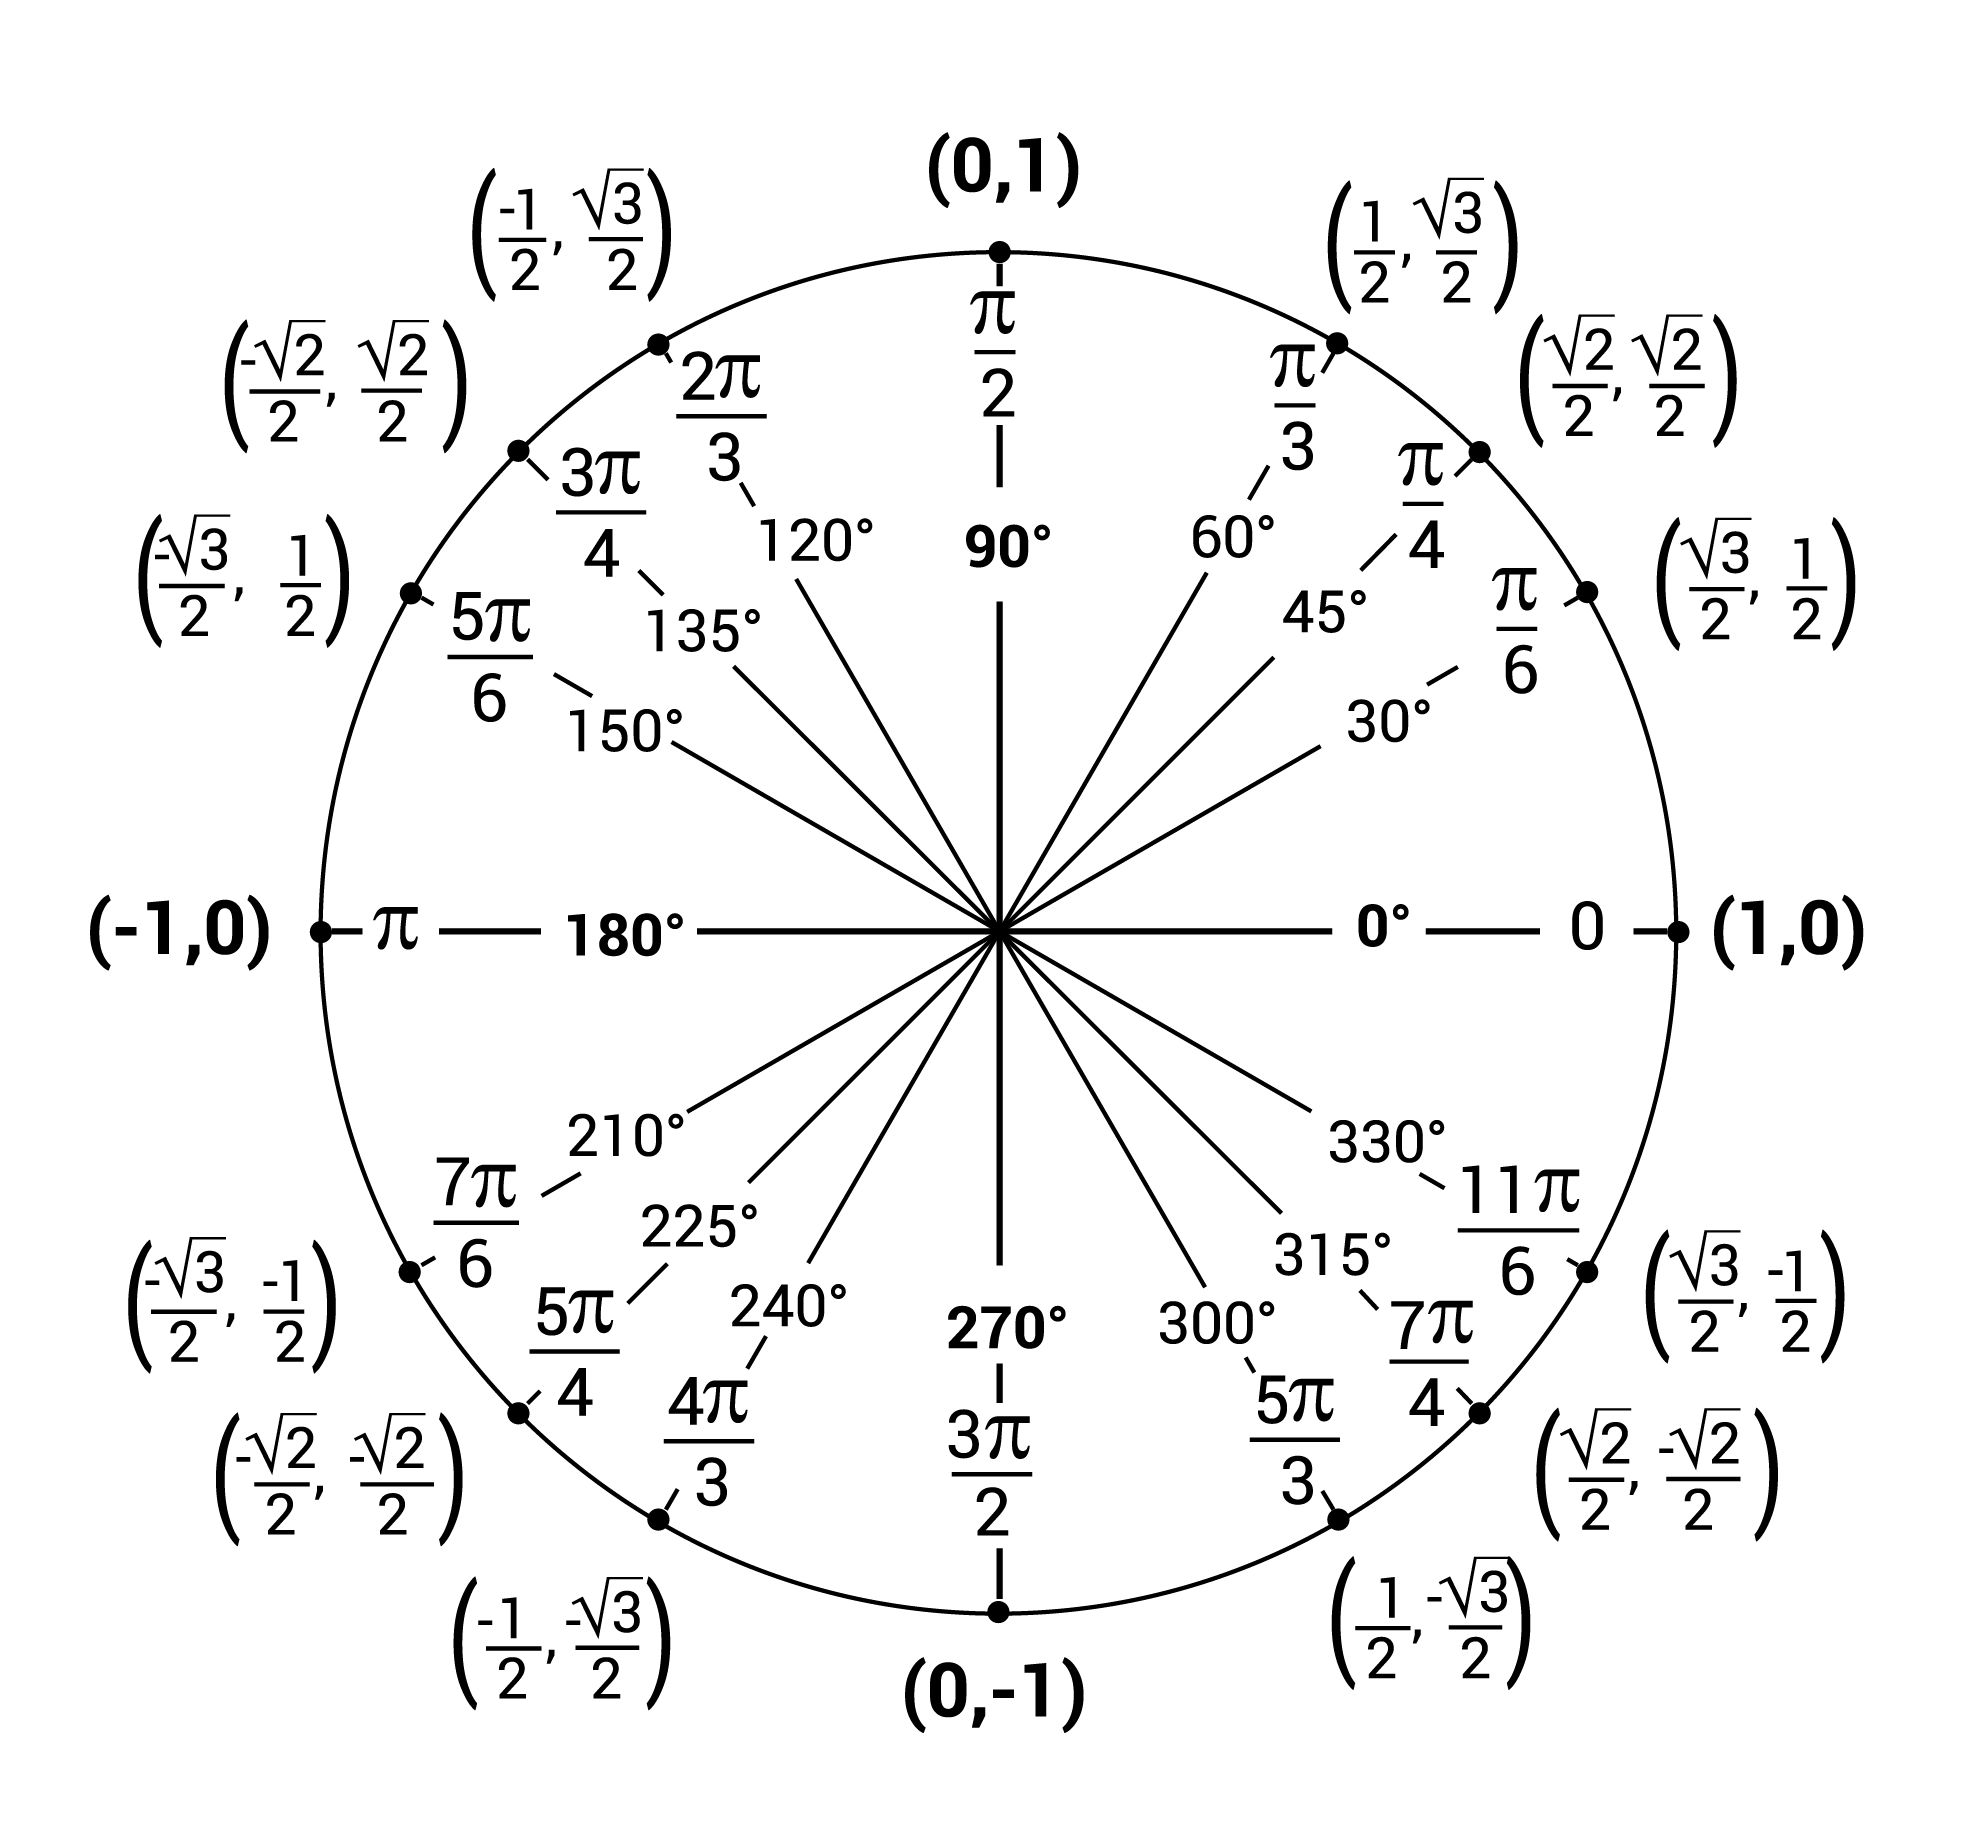
\includegraphics[width=6cm, height=6cm]{unit-circle.png}
\subsubsection{Trigonometric Identities}

\begin{center}
    \begin{tabular}{  p{5cm}  p{5cm} }
        $\csc x = \frac{1}{\sin x }$ & 
        $\sec x = \frac{1}{\cos x }$ \T \\
        
        $\cot x = \frac{1}{\tan x }$ & 
        $\tan x = \frac{sin x}{\cos x }$ \T \\
        $\cot x = \frac{cos x}{\sin x }$ & 
        $\sin^2 x + cos^2 = 1$ \T \\

\end{tabular}
\end{center}
\vspace{1cm}
\section{Misc}
\subsection{LaTeX examples}
$(\frac{f(x)}{g(x)})$
\end{document}
